\documentclass{beamer}

\usepackage[czech]{babel}
\usepackage[utf8]{inputenc}
\usepackage[T1]{fontenc}
\usepackage{lmodern}
\usepackage{datetime}
\usepackage{tikz}
\usepackage{amssymb}
\usepackage{bbding}
\usepackage{tabularx}
\usepackage{wrapfig}
\usepackage{xcolor}

\usetikzlibrary{shadows}

\definecolor{sourcesclr}{rgb}{.38,.38,.38}

% Themes: http://www.hartwork.org/beamer-theme-matrix/
\mode<presentation>{\usetheme{Madrid}}
\usecolortheme{beaver}
\beamertemplatenavigationsymbolsempty 
\setbeamertemplate{title page}[default][colsep=0bp,rounded=true]
\setbeamertemplate{itemize items}{$\bullet$}
\setbeamercolor*{item}{fg=black}
\setbeamertemplate{enumerate item}[default]
\newcommand{\Has}{\textcolor{green}{\CheckmarkBold}}
\newcommand{\NoHas}{\textcolor{red}{\XSolidBrush}}
\newcommand{\It}{\textit}  % kurzíva
\newcommand{\B}{\textbf} %tučné písmo
\newcommand{\U}{\underline}  % podtržené písmo
\newcommand{\sectsel}[1]{\U{\B{#1}}}
\newcommand{\srctext}[1]{{\fontsize{7}{9}\selectfont\textcolor{sourcesclr}{#1}}}

\newenvironment<>{positiveblock}[1]{%
  \begin{actionenv}#2%
      \def\insertblocktitle{#1}%
      \par%
      \mode<presentation>{%
        \setbeamercolor{block title}{fg=white,bg=green!20!black}
       \setbeamercolor{block body}{fg=black,bg=green!40}
       \setbeamercolor{itemize item}{fg=green!20!black}
       \setbeamertemplate{itemize item}[triangle]
     }%
      \usebeamertemplate{block begin}}
    {\par\usebeamertemplate{block end}\end{actionenv}}

\newenvironment<>{negativeblock}[1]{%
  \begin{actionenv}#2%
      \def\insertblocktitle{#1}%
      \par%
      \mode<presentation>{%
        \setbeamercolor{block title}{fg=white,bg=red!20!black}
       \setbeamercolor{block body}{fg=black,bg=red!20}
       \setbeamercolor{itemize item}{fg=red!20!black}
       \setbeamertemplate{itemize item}[triangle]
     }%
      \usebeamertemplate{block begin}}
    {\par\usebeamertemplate{block end}\end{actionenv}}

\author{Vojtěch Boček}
\institute[vbocek@gmail.com]{Faculty of Informatics, Masaryk University}
\title{MultiROM}
\subtitle{The multiboot modification for Android devices}
\date[]{}

\setbeamerfont{sections}{size=\fontsize{8}{9}\selectfont}

\begin{document}


%\frame{\titlepage}


\begin{frame}[plain]
    \begin{center}
        \begin{figure}[H]
        \includegraphics[width=320px]{img/play_promo.png}
        \end{figure}
        \vspace{8mm}
        Vojtěch Boček\\
        \vspace{1mm}
        \srctext{Faculty of Informatics, Masaryk University}
    \end{center}
\end{frame}

\begin{frame}[plain]
    \begin{center}
    \includegraphics[width=150px]{img/android.jpg}
    \end{center}
    \pause
    \begin{columns}
    \column{.16\textwidth}
        \begin{center}
        \includegraphics[width=50px]{img/cm.png}
        \end{center}
    \column{.16\textwidth}
        \begin{center}
        \includegraphics[width=50px]{img/omni.png}
        \end{center}
        \pause
    \column{.16\textwidth}
        \begin{center}
        \includegraphics[width=50px]{img/ubuntu.png}
        \end{center}
    \column{.16\textwidth}
        \begin{center}
        \includegraphics[width=50px]{img/firefox.png}
        \end{center}
    \column{.16\textwidth}
        \begin{center}
        \includegraphics[width=50px]{img/sailfish.png}
        \end{center}
        \pause
    \column{.16\textwidth}
        \begin{center}
        \includegraphics[width=50px]{img/arch.png}
        \end{center}
    \end{columns}
\end{frame}

\begin{frame}
    \frametitle{MultiROM}
    \begin{columns}
    \column{.48\textwidth}
    \vspace{-10mm}
    \begin{itemize}
        \item multiple operating systems at once -- \It{multiboot}
        \item supports many different operating systems
        \item easy to use
    \end{itemize}
    \column{.48\textwidth}
    \vspace{-5mm}
    \begin{figure}[H]
    \includegraphics[width=170px]{../img/dragon.png}
    \end{figure}
%     \begin{figure}[H]
%     \begin{tikzpicture}
%         \node[drop shadow={shadow xshift=.8ex,shadow yshift=-.8ex},fill=white,draw] at (0,0) { \includegraphics[width=120px]{../img/boot_manager.png}};
%     \end{tikzpicture}
%     \end{figure}
    \end{columns}
\end{frame}

\begin{frame}
    \vspace{-2.5ex}
    \begin{beamercolorbox}[wd=\paperwidth,ht=2.5ex,dp=1.125ex,center=true]{palette quaternary}%
    \usebeamerfont{sections}
    \sectsel{1. Boot manager} | 2. Modified recovery | 3. Kexec-hardboot patch | 4. Android app
    \end{beamercolorbox}
    \vspace{-1.5ex}

    \frametitle{Boot Manager}
    \begin{columns}
    \column{.48\textwidth}
    \begin{itemize}
        \item shows up during boot
        \item lets user choose which system to boot
        \item contains most of the code related to multibooting
        \item can automagically boot pre-selected system
    \end{itemize}
    \vspace{10mm}

    \column{.48\textwidth}
    \begin{figure}[H]
    \begin{tikzpicture}
        \node[drop shadow={shadow xshift=.8ex,shadow yshift=-.8ex},fill=white,draw] at (0,0) { \includegraphics[width=120px]{../img/boot_manager.png}};
    \end{tikzpicture}
    \end{figure}
    \end{columns}
\end{frame}

\begin{frame}
    \vspace{-2.0ex}
    \begin{beamercolorbox}[wd=\paperwidth,ht=2.5ex,dp=1.125ex,center=true]{palette quaternary}%
    \usebeamerfont{sections}
    1. Boot manager | \sectsel{2. Modified recovery} | 3. Kexec-hardboot patch | 4. Android app
    \end{beamercolorbox}
    \vspace{-1.5ex}

    \frametitle{Modified recovery}
    \begin{columns}
    \column{.48\textwidth}
    \begin{itemize}
        \item originaly intended for recovery of the main system
        \item management of the secondary systems
        \item MultiROM settings
        \item based on the TWRP open-source project
    \end{itemize}
    \vspace{10mm}

    \column{.48\textwidth}
    \begin{figure}[H]
    \begin{tikzpicture}
        \node[drop shadow={shadow xshift=.8ex,shadow yshift=-.8ex},fill=white,draw] at (0,0) { \includegraphics[width=120px]{../img/recovery2.png}};
    \end{tikzpicture}
    \end{figure}
    \end{columns}
\end{frame}

\begin{frame}
    \vspace{-12.4ex}
    \begin{beamercolorbox}[wd=\paperwidth,ht=2.5ex,dp=1.125ex,center=true]{palette quaternary}%
    \usebeamerfont{sections}
    1. Boot manager | 2. Modified recovery | \sectsel{3. Kexec-hardboot patch} | 4. Android app
    \end{beamercolorbox}
    \vspace{13.0ex}

    \frametitle{Kexec-hardboot patch}
    \begin{itemize}
        \item Linux kernel modification
        \item starts new kernel from the already running one
        %\item nepřepíše jádro uložené v boot sektoru
        \item \B{enables multiboot on devices as limited as Android phones and tablets}
    \end{itemize}
\end{frame}

\begin{frame}
    \vspace{-3.7ex}
    \begin{beamercolorbox}[wd=\paperwidth,ht=2.5ex,dp=1.125ex,center=true]{palette quaternary}%
    \usebeamerfont{sections}
    1. Boot manager | 2. Modified recovery | 3. Kexec-hardboot patch | \sectsel{4. Android app}
    \end{beamercolorbox}
    \vspace{-1.0ex}

    \frametitle{Android application}
    \begin{columns}
    \column{.48\textwidth}
    \begin{itemize}
        \item installs and updates all parts of MultiROM
        \item can rename and delete secondary systems
        \item boot directly into one of the systems
    \end{itemize}
    \vspace{10mm}

    \column{.48\textwidth}
    \begin{figure}[H]
    \begin{tikzpicture}
        \node[drop shadow={shadow xshift=.8ex,shadow yshift=-.8ex},fill=white,draw] at (0,0) { \includegraphics[width=120px]{../img/app_main2.png}};
    \end{tikzpicture}
    \end{figure}
    \end{columns}
\end{frame}

% BOOT MENUp
% to stejne na N5, tam boot android
% N7 - recovery, boot android
% n5 - ukazat nabootovanou rom, reboot do ubuntu
% n7 - ukazat app a widget
% n5 - ukazat ubuntu

\begin{frame}
    \begin{center}
        {\Large *\It{Probably a}\,live demo!* }
        \vspace{5mm}
        \begin{figure}[H]
        \includegraphics[width=0.4\textwidth]{../img/kocka.png}
        \end{figure}
    \end{center}
    \vspace{15mm}
    \srctext{Author: Ketrina Yim (draguunthor.deviantart.com)}
\end{frame}

\begin{frame}
    \frametitle{Project status}
    \begin{itemize}
        \item generally useful utility
        \item 4 supported devices and several unofficial ports done by community
        \item over 30 000 active installations
        \item other developers are using MultiROM and its parts
        \item successful crowdfunding campaign
        \item participation on several student competitions
    \end{itemize}
\end{frame}

\begin{frame}
    \frametitle{Obstacles}
    \begin{itemize}
        \item the platform is very fragmented
        \begin{itemize}
            \item no BIOS/ACPI/UEFI -> separate kernels for each device
            \item each device is different, especially across different vendors
            \item even ROMs can be quite different at low-level
        \end{itemize}
        \pause
        \vspace{3mm}
        \item hidden bugs
        \vspace{3mm}
        \pause
        \item people are... \It{people}
    \end{itemize}
\end{frame}



\begin{frame}
    \begin{center}
        {\Large Thank you for your attention!}

        \vspace{2mm}

        \begin{figure}[H]
        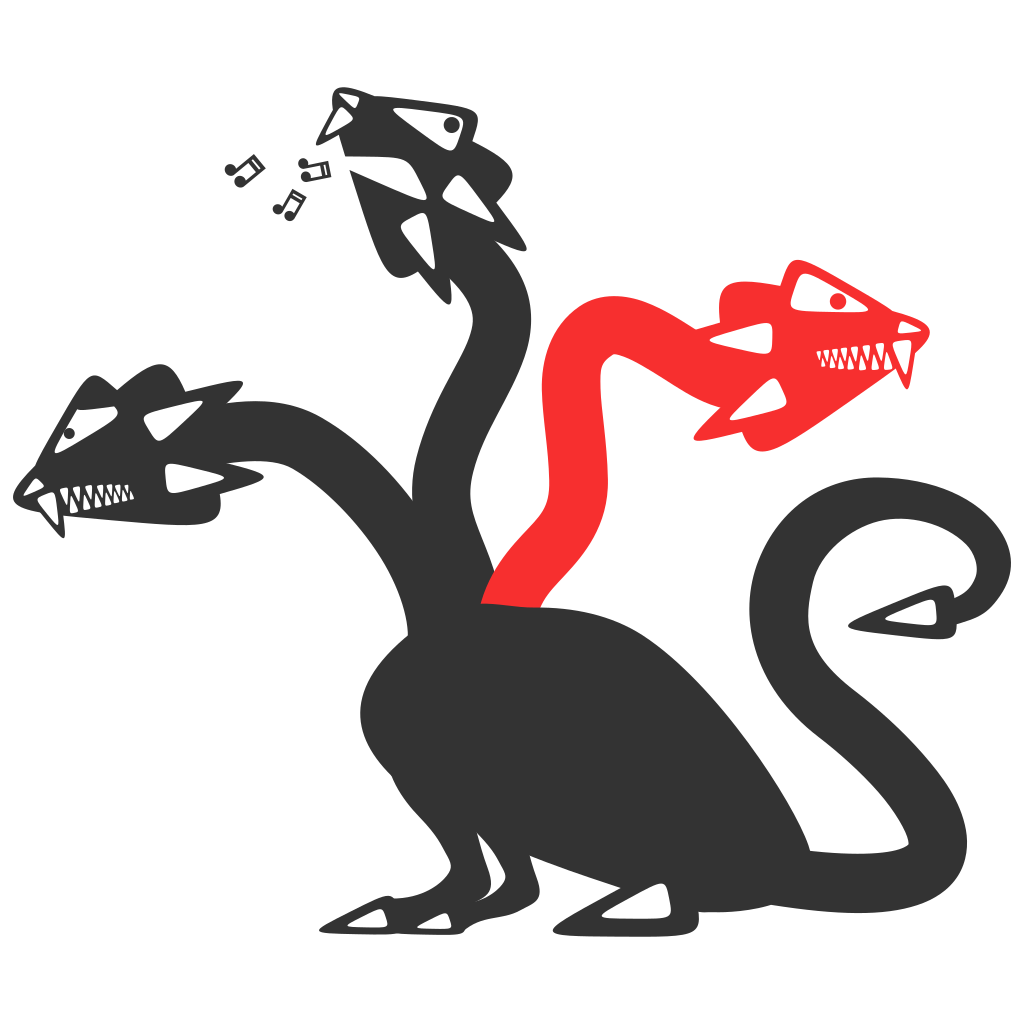
\includegraphics[width=0.45\textwidth]{../img/dragon_full.png}
        \end{figure}
    \end{center}
    \srctext{Image sources:}
    \begin{itemize}
        \item[]\hspace{-5mm}\srctext{\B{Miri the Hydra:} me.}
        \item[]\hspace{-5mm}\srctext{\B{Schrödinger's cat:} \url{http://draguunthor.deviantart.com/art/Schrodinger-s-Cat-163302750}}
        \item[]\hspace{-5mm}\srctext{\B{All the OS logos:} The internets, you don't really care if I put sources in here or not \^\^.}
    \end{itemize}
\end{frame}

\end{document}
